%---------------------------------- Exp1 : 72direct -------------------------------
\begin{frame}[allowframebreaks]{Experiment 1 : Proof of concept using DiRect with Zellij}
    \begin{block}{Experimental setup}
        23 hours of run : 72 complete iterations using direct implementation of Zellij.\\
        Fixed HP : 1 epochs by training\\
        
    \end{block}
    \begin{columns}
    
        \begin{column}[t]{0.6\textwidth}
            \begin{block}{Variable one by one}
            
                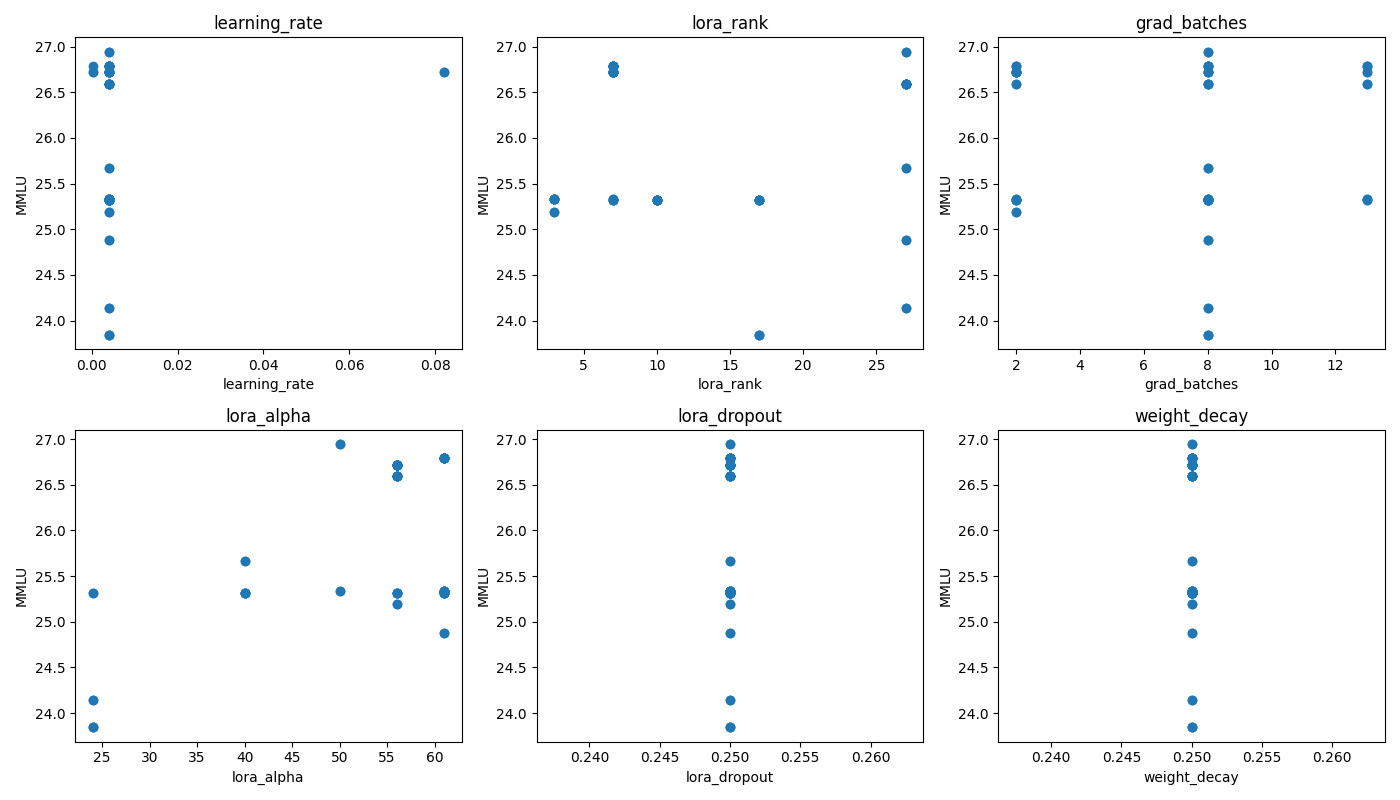
\includegraphics[width = 7.5cm]{imgs/individual_results.png}
            
            \end{block}   
        \end{column}

        \begin{column}[t]{0.4\textwidth}
            \begin{block}{Convergence}
            Best MMLU result : 26,94\%
            
        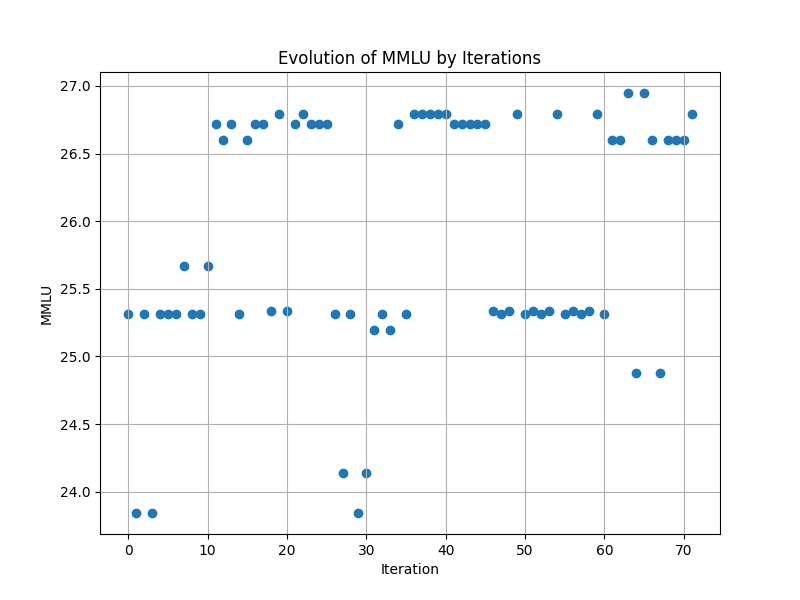
\includegraphics[width = 5cm]{imgs/mmlu_evolution.png}
            
            \end{block}  
            
        \end{column}
    \end{columns}    
\end{frame}

%---------------------------------- Optimization -------------------------------
\begin{frame}[allowframebreaks]{Experiment 2 : First step with Bayesian Optimization}
    \begin{block}{Experimental setup}
        50 complete iterations with BoTorch implementation\\
        Hardware : single node with 4*A100 40G
    \end{block}

    \begin{block}{Gaussian Process parameter}
    \begin{itemize}
        \item Acquisition function : Log EI
        \item model : MixedSingleTaskGP
        \item likelihood : ExactMarginalLogLikelihood
    \end{itemize}
        
    \end{block}

    \framebreak
    
    \begin{columns}
    
        \begin{column}[t]{0.6\textwidth}
            \begin{block}{Variable one by one}
            
                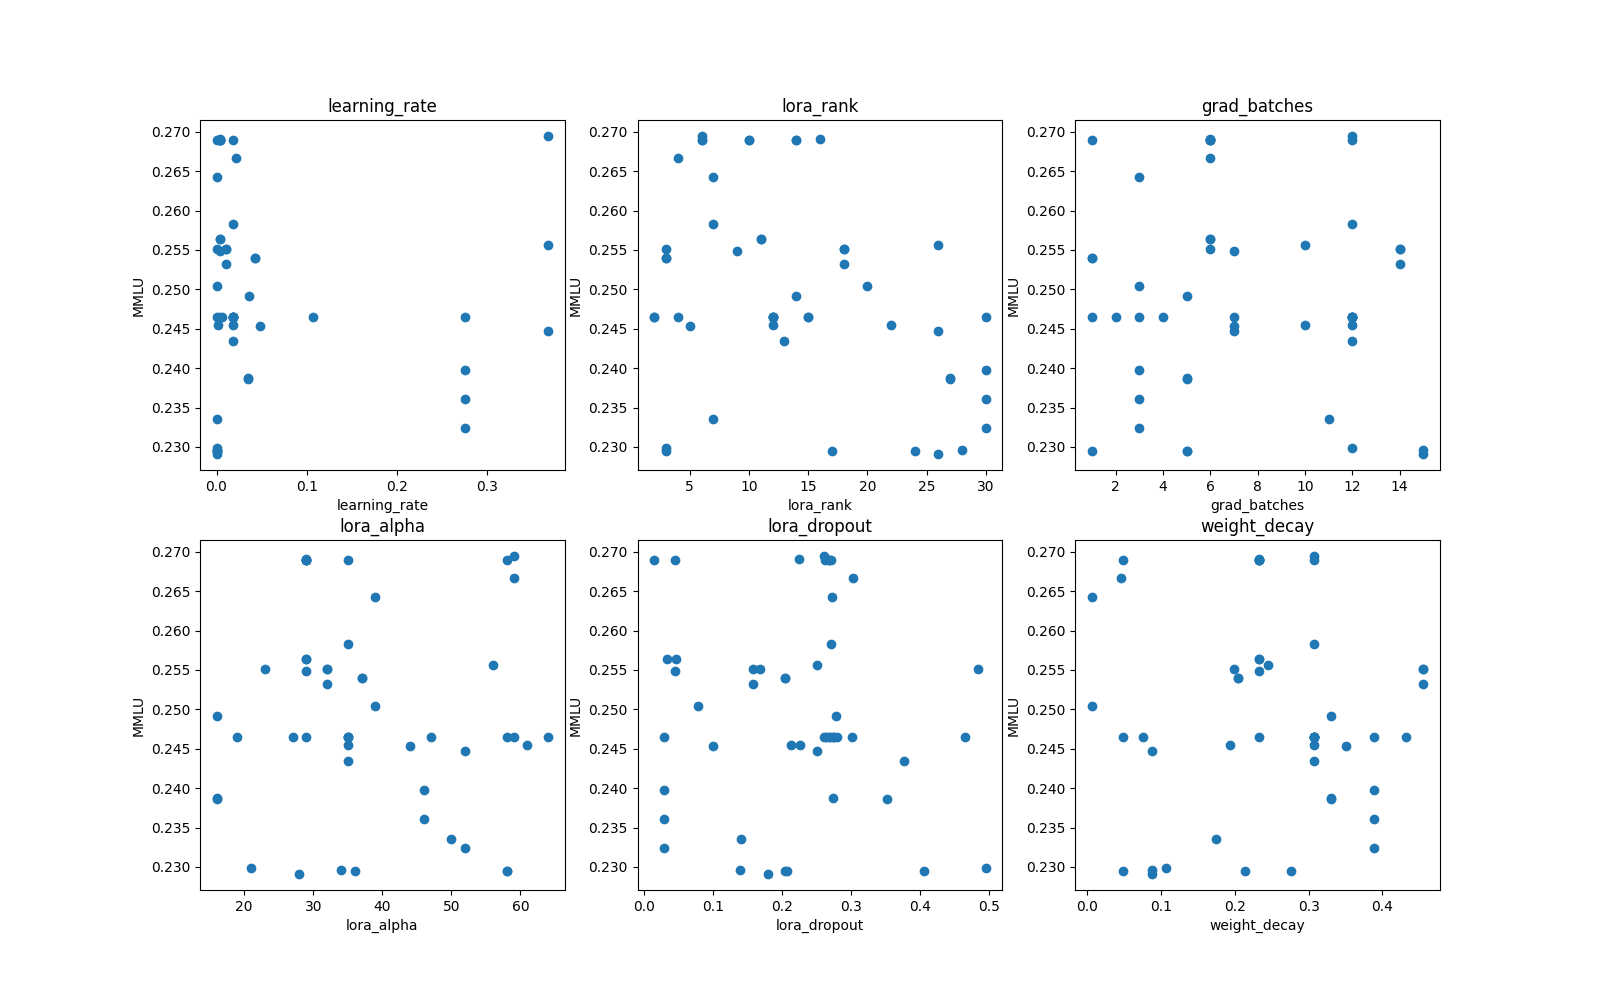
\includegraphics[width = 7.5cm]{imgs/exp2-bo_individual.png}
            
            \end{block}   
        \end{column}

        \begin{column}[t]{0.4\textwidth}
            \begin{block}{Convergence}
            Best MMLU result : 26,94\%
            
        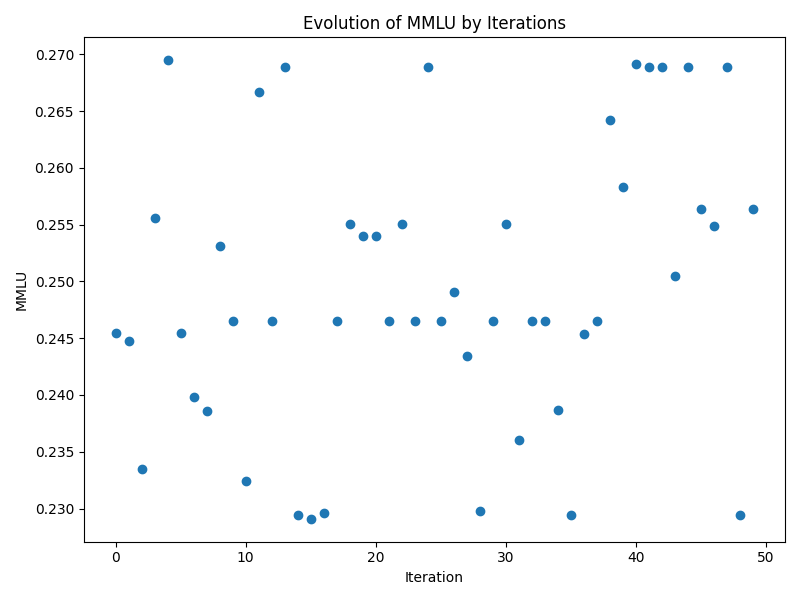
\includegraphics[width = 5cm]{imgs/exp2-bo_mmlu.png}
        TO DO : look if there is convergence at some point
            
            \end{block}  
            
        \end{column}
    \end{columns}    
\end{frame}

%---------------------------------- Optimization -------------------------------
\begin{frame}[allowframebreaks]{Experiment 3 : Bayesian Optimization with Latin Hypercube Sampling}


    \begin{columns}
    
        \begin{column}[t]{0.6\textwidth}
    \begin{block}{Experimental setup}
        57 complete iterations with BoTorch implementation\\
        Training : one epoch on alpaca cleaned dataset\\
        Evaluation : Hellaswag dataset\\
        Hardware : single node with 4*A100 40G
    \end{block}

    \begin{block}{Gaussian Process parameter}
    \begin{itemize}
        \item Acquisition function : Log EI
        \item model : MixedSingleTaskGP
        \item likelihood : ExactMarginalLogLikelihood
    \end{itemize}
        
    \end{block}  
        \end{column}

        \begin{column}[t]{0.4\textwidth}
            \begin{block}{Convergence}
            Best Hellaswag result : 53,02\%
            
        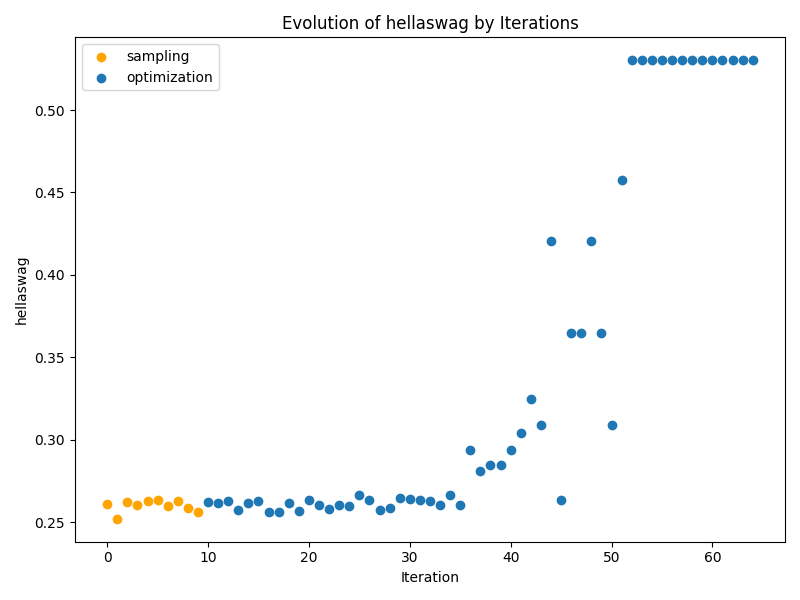
\includegraphics[width = 5cm]{imgs/exp03/score_by_iteration.png}
            
            \end{block}  
            
        \end{column}
    \end{columns}    

    \framebreak
    
    \begin{columns}
    
        \begin{column}[t]{0.45\textwidth}
            \begin{block}{Variable one by one}
            
                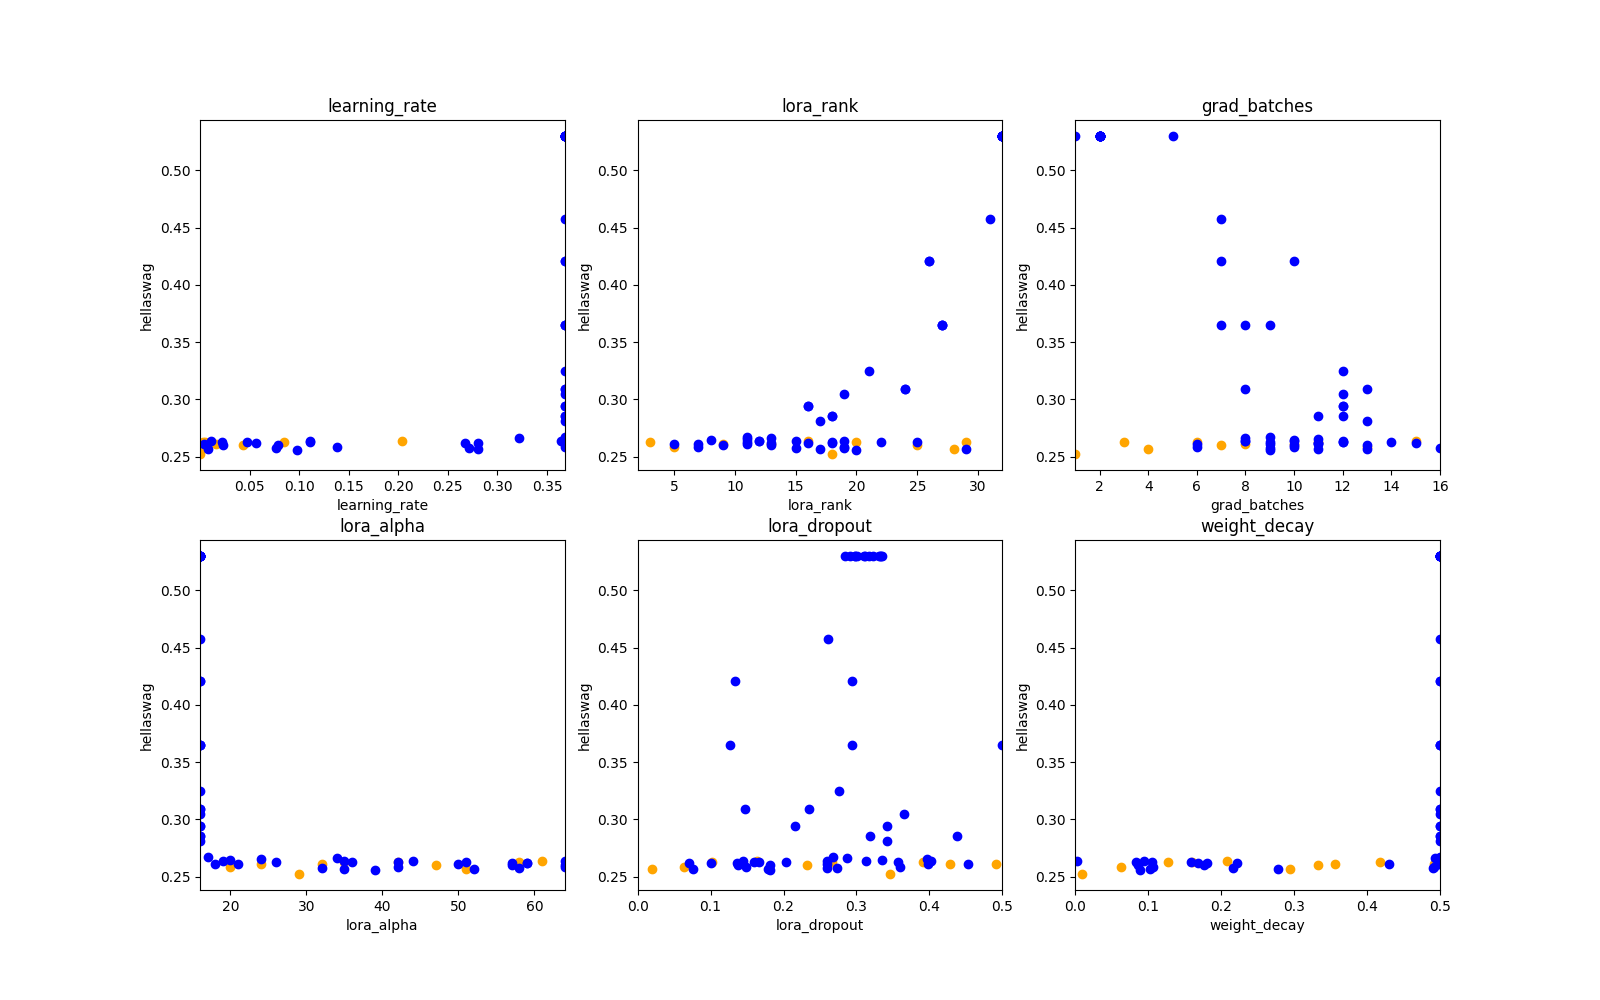
\includegraphics[width = 7cm]{imgs/exp03/score_by_variable.png}
            
            \end{block}   
        \end{column}

        \begin{column}[t]{0.45\textwidth}
            \begin{block}{Variable iteration}
            
        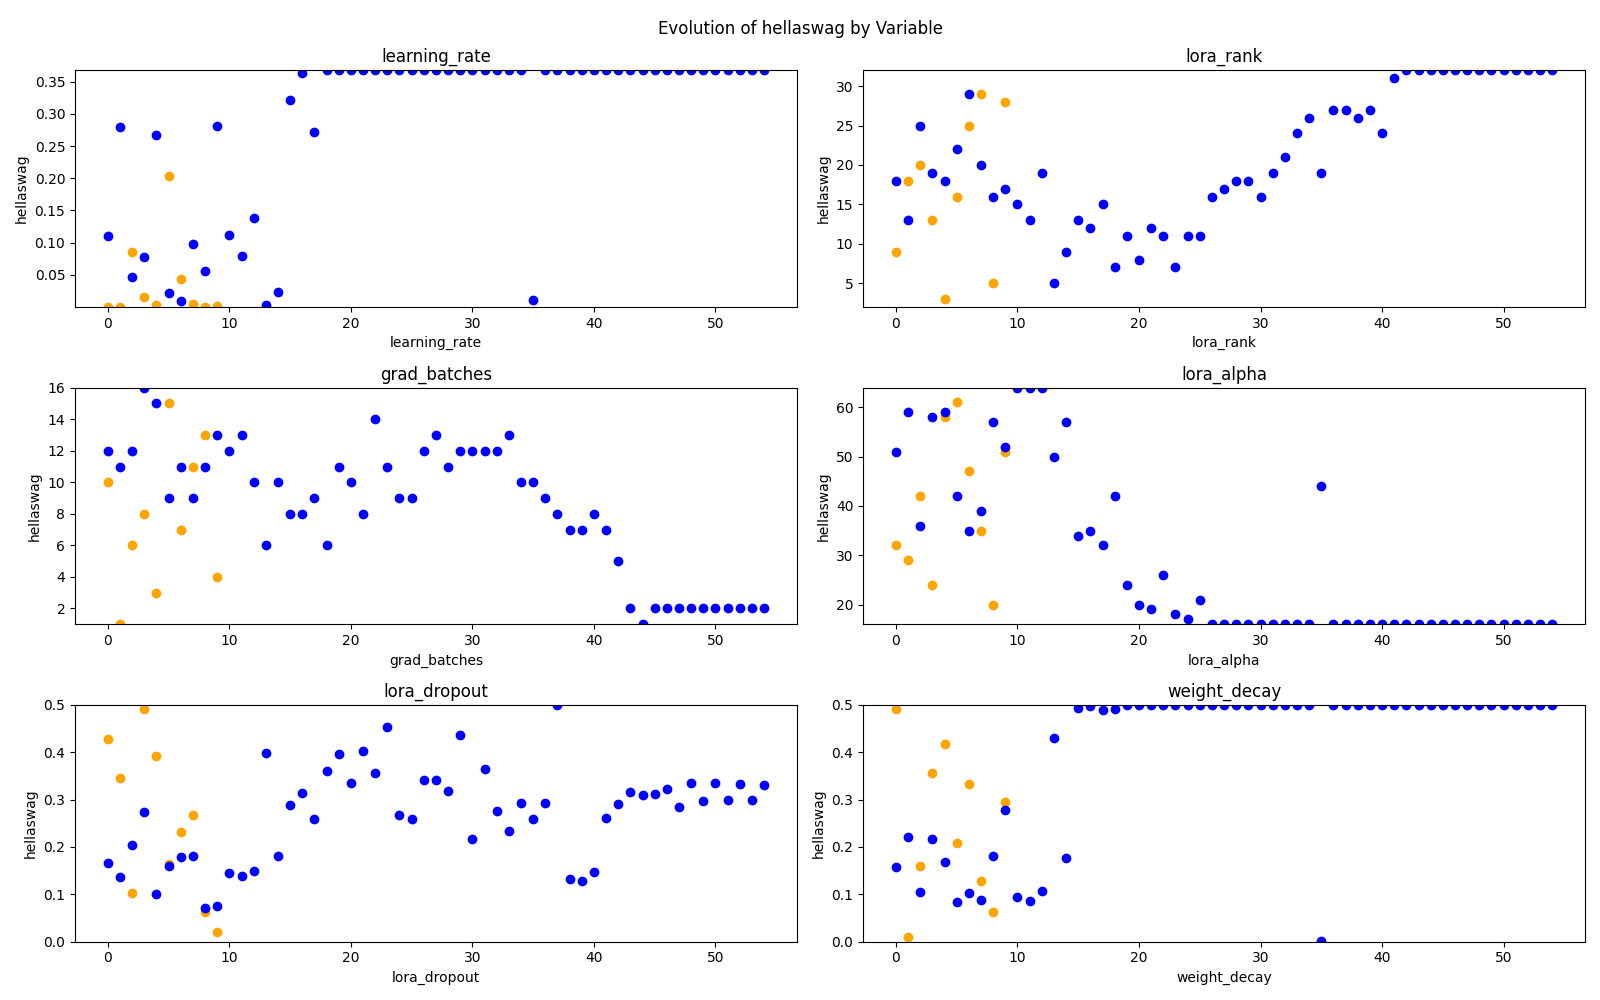
\includegraphics[width = 7cm]{imgs/exp03/variable_over_time.png}
            
            \end{block}  
            
        \end{column}
    \end{columns}    

    \begin{block}{Results}
        Need to enlarge search space, since 5 hyperparameters are constrained by bounds.
    \end{block}
    
\end{frame}